% METODOLOGIA------------------------------------------------------------------

\chapter{Metodologia}
\label{chap:metodologia}

% LEMBRAR DE NÃO FALAR DO SILVIO AQUI

A metodologia empregada neste trabalho está organizada nos seguintes passos principais:

\begin{description}
\item[Etapa 1] Aquisição da base de vídeos UCF50 - Action Recognition Data Set \citeauthor{reddy2013recognizing}.
\item[Etapa 2] Aplicação das 14 distorções descritas na Seção~\ref{sec:ataques} sobre a base.
\item[Etapa 3] Geração das assinaturas utilizando os algoritmos baseados em diferença de quadro, gradientes, medida ordinal, quadros de cena, padrão binário por região e wavelets, descritos no Capítulo~\ref{chap:revisao}.
\item[Etapa 4] Realização do procedimento de comparação de um conjunto de treinamento das assinaturas, a fim de definir um limiar para classificação.
\item[Etapa 5] Realização do procedimento de comparação de um conjunto de testes das assinaturas, a partir dos limiares obtidos na Etapa 4.
\item[Etapa 5] Análise comparativa dos resultados obtidos a partir da Etapa 4. Os resultados desta etapa serão discutidos em detalhes no próximo capítulo.
\end{description}

As seções a seguir detalham como esses passos serão realizados.

\section{Definição e Obtenção da Base de Vídeos}
\label{sec:database}

Para a realização dos experimentos desta monografia, foi escolhida a base de vídeos UCF50 - Action Recognition Data Set \citeauthor{reddy2013recognizing}, que é comumente utilizada em projetos de reconhecimento de movimento humano. Ela foi escolhida pela quantidade de vídeos que contém, além de sua licença de livre utilização.

Ela está segmentada em 50 categorias diferentes que representam ações do quotidiano, como por exemplo ciclismo, natação, caminhada com o cachorro, TaiChi, etc. Dentro de cada categoria, há pelo menos 4 vídeos pertencentes a uma mesma gravação, apresentando assim os mesmos personagens, fundo e ponto de vista. A fim de reduzir o número de vídeos que apresentam o mesmo conteúdo, foram selecionados apenas o primeiro vídeo de cada grupo.

A base original é composta de 6.681 vídeos com duração média entre 3 a 9 segundos e após a seleção descrita no parágrafo anterior, restaram 1.264 vídeos. Para cada vídeo selecionado foram aplicadas as distorções descritas na Seção~\ref{sec:ataques}, totalizando 18.960 itens, sendo destes, 17.696 vídeos resultantes das distorções. A Figura~\ref{fig:exemplos} apresenta alguns exemplos de vídeos da base.

\begin{figure}
    \centering
    \caption{Exemplos de vídeos retirados da base. O primeiro mostra um jogo de baseball, o segundo mostra uma criança fazendo malabarismo, o terceiro mostra uma competição de levantamento de pesos}
    \label{fig:exemplos}
    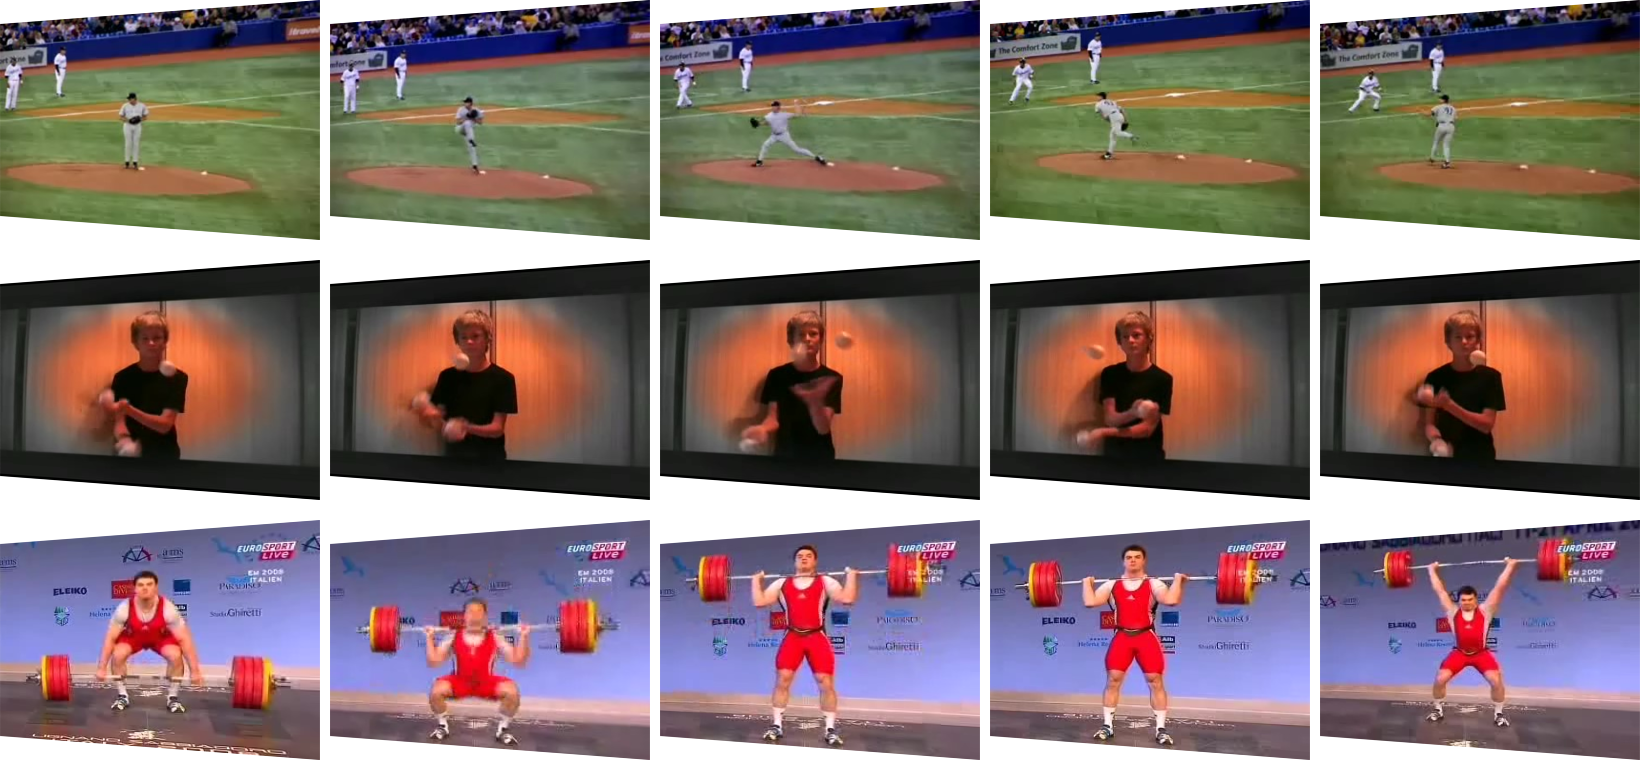
\includegraphics[width=0.8\textwidth]{dados/figuras/exemplos.png}
\end{figure}

\section{Aplicação das Distorções}
\label{sec:met-distorcoes}

Para a criação de um conjunto de cenários de treinamento e teste, foram aplicadas as 14 distorções descritas na Seção~\ref{sec:ataques} sobre os 1.264 vídeos selecionados da base UCF50. Estes cenários propiciam a avaliação do desempenho das diferentes assinaturas revisitadas neste trabalho quanto à robustez e unicidade quando os vídeos são submetidos a diferentes tipos de distorções. A fim de garantir a reprodutibilidade do experimento, os parâmetros utilizados para a aplicação de cada uma das distorções são explicitados na Tabela~\ref{tab:params}.

\begin{table}[h]
\centering
\caption{Parâmetros usados na aplicação das distorções}
\label{tab:params} \begin{tabular}{|l|l|} \hline
\textbf{Distorção}                                                                & \textbf{Parâmetros}                                                                                                      \\ \hline
\multicolumn{1}{|l|}{Adição de texto e legendas}                                  & \multicolumn{1}{l|}{}                                                                                                    \\ \hline
\multicolumn{1}{|l|}{Adição de Marca D'água}                                      & \multicolumn{1}{l|}{\begin{tabular}[c]{@{}l@{}}Texto: "Copyright"\\ Tamanho da fonte: 20\\ Opacidade: 65\%\end{tabular}} \\ \hline
\multicolumn{1}{|l|}{Adição de Quadro ou Bordas}                                  & \multicolumn{1}{l|}{Tamanho da borda: 25 pixels}                                                                         \\ \hline
\multicolumn{1}{|l|}{Redimensionamento da Altura e Largura dos Vídeos para Maior} & \multicolumn{1}{l|}{\begin{tabular}[c]{@{}l@{}}Fator de redimensionamento: 2\\ Mantém aspect ratio: sim\end{tabular}}    \\ \hline
\multicolumn{1}{|l|}{Eliminação de uma faixa ou região dos quadros}               & \multicolumn{1}{l|}{}                                                                                                    \\ \hline
\multicolumn{1}{|l|}{Inversão/espelhamento}                                       & \multicolumn{1}{l|}{Sentido: horizontal}                                                                                 \\ \hline
\multicolumn{1}{|l|}{Rotação}                                                     & \multicolumn{1}{l|}{10 graus}                                                                                            \\ \hline
\multicolumn{1}{|l|}{Desfoque/borrado}                                            & \multicolumn{1}{l|}{\begin{tabular}[c]{@{}l@{}}Tipo: gaussiano\\ Sigma: 3\end{tabular}}                                  \\ \hline
\multicolumn{1}{|l|}{Inversão das cores}                                          & \multicolumn{1}{l|}{}                                                                                                    \\ \hline
\multicolumn{1}{|l|}{Alteração das compressão dos quadros do vídeo}               & \multicolumn{1}{l|}{Compressão utilizada: JPEG}                                                                          \\ \hline
\multicolumn{1}{|l|}{Aceleração do vídeo 1}                                       & \multicolumn{1}{l|}{Aumento da velocidade em 50\%}                                                                       \\ \hline
\multicolumn{1}{|l|}{Aceleração do vídeo 2}                                       & \multicolumn{1}{l|}{Aumento da velocidade em 25\%}                                                                       \\ \hline
Remoção de quadros                                                                &                                                                                                                          \\ \hline
\end{tabular}
\end{table}

\section{Geração das Assinaturas}
\label{sec:met-assinaturas}

\section{Comparações de Assinaturas para Treinamento}
\label{sec:met-comparacao-treinamento}

\section{Comparações de Assinaturas para Testes}
\label{sec:met-comparacao-testes}


\section{Análise dos Resultados}
\label{sec:met-analise}


% Foi escolhida a linguagem Python (versão 2.7.12) para a implementação dos algoritmos por ser multiplataforma e  por sua simplicidade na integração com bibliotecas de alta-performance implementadas em linguagens de baixo nível (C). Isto foi importante pois serão utilizadas as bibliotecas \textit{OpenCV} (versão 3.0.0) e \textit{NumPy} (versão 1.12.1) para manipulação e operação de imagens.

% Para a compilação da base de vídeos foi utilizada a biblioteca MagicImage (versão 7.0.7-8-Q16-x64 - Windows), que incluí os programas \textit{convert} e \textit{ffmpeg}, utilizados para conversão de formatos, aplicação de distorções e transformações de vídeo e imagem respectivamente.

% \section{Definição e Implementação do método de comparação}


% \textbf{[EM DESENVOLVIMENTO]}

% pegar base de assinaturas distrocidas, e para cada distorçao, calcular a distancia para todas as assinaturas originais

% pegar as duas menores distancias para cada distorçao de cada vídeo

% se a dif do primeiro colocado (primera distancia) for diferente o suficiente para o segundo colocado , entao podemos assumir (podemos?) que encontramos a assinatura do vídeo original

% EMBASAR ESSAS PARADAS LOUCAS

% \section{Validação das implementações}

% Antes de realizar-se qualquer experimento, é necessário que os algoritmos implementados passem por uma etapa de validação que consiste em comparar seus resultados com os dos artigos de base. Para isso serão revisados os artigos dos quais os algoritmos foram retirados, além de códigos disponibilizados através destes trabalhos.

% A validação ocorrerá em duas etapas:

% \begin{enumerate}
% \item teste de software;
% \item comparação das saídas dos algoritmos implementados para o trabalho e as implementações originais, dada a mesma entrada.
% \end{enumerate}

% \section{Definição dos Experimentos}
% \label{sec:definicaoexperimentos}